\documentclass[letterpaper,12pt,fleqn]{article}
\usepackage{matharticle}
\usepackage{tikz}
\pagestyle{plain}
\begin{document}

\begin{center}
  \large
  Math-71 Sections 9, 11, 12

  \Large
  Practice Exam \#1
\end{center}

\vspace{0.5in}

This exam will be closed book and notes. You may use a scientific calculator; however, no other electronics are allowed.  You
may also use the instructor-provided cheatsheet.  Show all work; there is no credit for guessed answers.  Simplify your answers
unless told otherwise.  In particular, all answers should contain no negative or rational exponents.  All numerical answers
should be in exact form unless you are specifically asked for a decimal value.

\vspace{0.25in}

\begin{enumerate}[left=0pt]
\item Consider the function:
  \[f(x)=\frac{x+5}{x^2+4x-5}\]
  \begin{enumerate}
  \item Evaluate:
    \[\lim_{x\to-5}f(x)\]
  \item Where is \(f(x)\) continuous?  Be sure to express your answer in interval notation.
  \end{enumerate}

  \bigskip

\item Consider the function:
  \[g(x)=\frac{\sqrt{x+1}-2}{x-3}\]
  \begin{enumerate}
  \item Evaluate:
    \[\lim_{x\to3}g(x)\]
  \item Where is \(g(x)\) continuous?  Be sure to express your answer in interval notation.
  \end{enumerate}

  \newpage

\item Consider the following function.  Assume that \(x=3\) is a vertical asymptote and that the domain extends to
  \(+\infty\).

  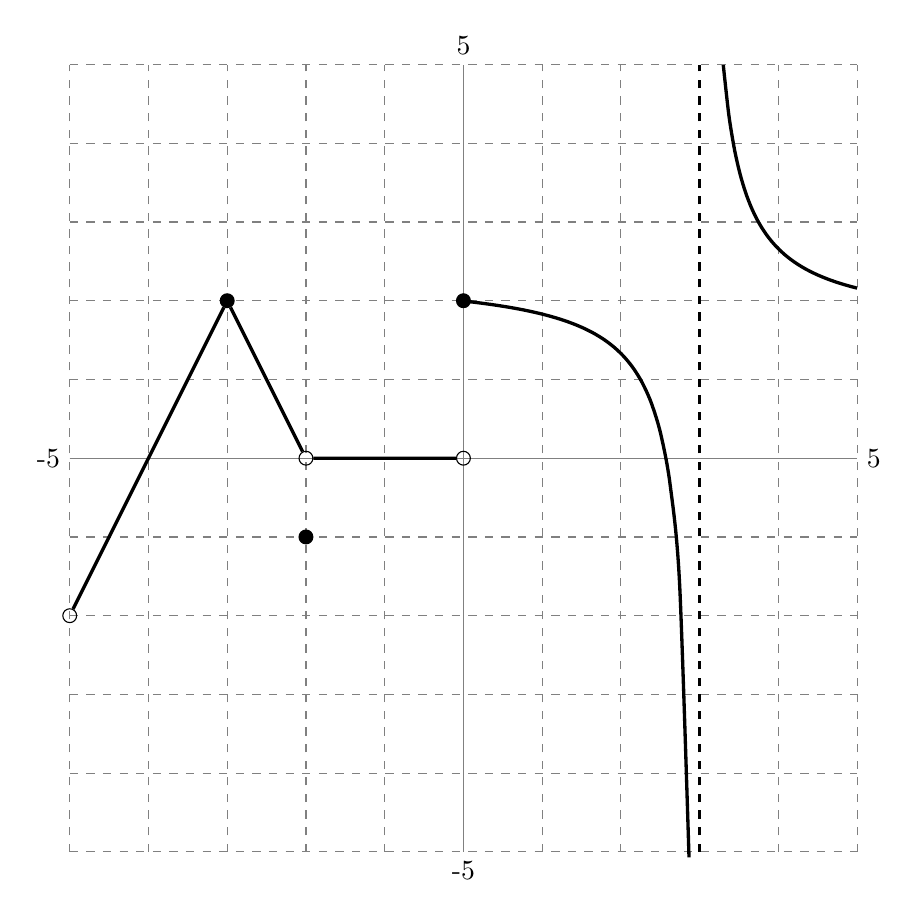
\begin{tikzpicture}[
      fillnode/.style={draw,circle,fill,inner sep=0pt,minimum size=5pt},
      opennode/.style={draw,circle,inner sep=0pt,minimum size=5pt},
    ]
    \draw [gray,dashed] (-5,-5) grid (5,5);
    \draw [help lines] (-5,0) to (5,0);
    \draw [help lines] (0,-5) to (0,5);
    \draw [dashed,very thick] (3,-5) -- (3,5);
    \node (A) [opennode] at (-5,-2) {};
    \node (B) [fillnode] at (-3,2) {};
    \node (C) [opennode] at (-2,0) {};
    \node (D) [fillnode] at (-2,-1) {};
    \node (E) [opennode] at (0,0) {};
    \node (F) [fillnode] at (0,2) {};
    \draw [very thick] (A) to (B) to (C) to (E);
    \draw [domain=0:2.865,smooth,very thick] plot ({\x},{2.33-1/abs{(\x-3)}});
    \draw [domain=3.3:5,smooth,very thick] plot ({\x},{1.66+1/abs{(\x-3)}});
    \node [left] at (-5,0) {-5};
    \node [right] at (5,0) {5};
    \node [below] at (0,-5) {-5};
    \node [above] at (0,5) {5};
  \end{tikzpicture}

  \begin{enumerate}
  \item Write down the three requirements for a function \(f(x)\) to be continuous at a point \(x=c\).
    \begin{enumerate}[label={\arabic*)}]
    \item
    \item
    \item
    \end{enumerate}
  \item For each discontinuity in the above function, list the \(x\) value at where the discontinuity occurs and indicate
    (with an `X') which of the three parts of the definition of continuity are violated.  Note that you may or may not use all
    of the rows and each point could violate multiple parts.

    \begin{tabular}{|p{0.5in}|c|c|c|}
      \hline
      \(x\) & (1) & (2) & (3) \\
      \hline
      & & & \\
      \hline
      & & & \\
      \hline
      & & & \\
      \hline
      & & & \\
      \hline
      & & & \\
      \hline
    \end{tabular}
  \end{enumerate}

  \newpage

\item Write down the definition of the derivative and the two characterizations that we discussed in class:
  \begin{description}
  \item {DEF:}
  \item {CHAR1:}
  \item {CHAR2:}
  \end{description}

  \bigskip

\item Consider the function:
  \[p(x)=-2x^3+3x^2-5x+10\]
  \begin{enumerate}
  \item Using the derivative rules, determine \(p'(x)\) in a step-by-step fashion.  You can combine multiple steps in each
    line; however, do not skip any steps.
  \item Where is \(p(x)\) continuous?  Be sure to express your answer in interval notation.
  \end{enumerate}

  \bigskip

\item Differentiate the following function:
  \[f(x)=2x^2+\frac{2}{x}+\sqrt{x}\]

  \bigskip

\item Differentiate the following function using the product rule:
  \[f(x)=(x^2+1)(x-2)\]

  \bigskip

\item Differentiate the following function using the quotient rule:
  \[f(x)=\frac{x+1}{2x^2-3}\]

  \bigskip

\item You have an urge to jump out of a perfectly good airplane with a parachute.  Unfortunately, your parachute fails.
  Your equation of motion that gives your height (in feet) at a given time \(t\) (in seconds) is:
  \[h(t)=10000-16t^2\]
  How fast are you going after 5 seconds?  Be sure that your answer includes the correct units.

  \bigskip

\item You work for the ACME Widget Factory.  The chief designer has come up with a revolutionary new widget design.  It is
  determined that the profit function (in dollars) for making \(x\) of these new widgets is:
  \[P(x)=0.01x^2+250x-1000\]
  The target production goal is 100 widgets.  Using marginal profit, estimate the difference in profit for making just 98
  widgets.  Be sure that your answer includes the correct units.
\end{enumerate}

\end{document}
